%% Chapter 3 — Control.
%%
%% Premise: the levers that work, and why they work — each maps to something that was rated.
%%
%% Rebuilt 2026-08-20 against curriculum/review-ch03.md. Four decisions drive the shape:
%%
%%   1. ORGANISED BY THE SIX RATED DIMENSIONS, not by a list of techniques. The old deck
%%      carried a "maps to" line under each technique, which is the best pedagogical device
%%      in the course and was being used as a footnote. Here the mapping IS the structure:
%%      walk Chapter 2's six dimensions and give the lever that steers each. Five have one.
%%      Harmlessness does not, and saying so explains refusal behaviour.
%%   2. One running example, a weak prompt this room would plausibly type, improved lever by
%%      lever: "Check my concrete mix design."
%%   3. The standing column is promoted out of the closing table onto each lever's frame, so
%%      a reader who leaves early still knows which claims were tested.
%%   4. Two frames are new because the old chapter had no equivalent and the room needs both:
%%      attaching a file or image, and which model is selected.
%%
%% Every headline is a full-sentence assertion. Ten of the old chapter's seventeen were
%% phrases, which throws away the one slide-design choice with converging experimental
%% support behind it.
%%
%% CLAUDE.md rule 5 governs every example: nothing is reproduced or paraphrased from any
%% vendor document. Every prompt, response and rubric row is synthetic and built on this
%% group's own domain.
\documentclass[aspectratio=169,11pt]{beamer}
\usetheme{UHTraining}
%% Shared preamble for the course decks.
\usepackage{uhcite}
\usepackage{uhslot}
\usepackage{amsmath}
\usetikzlibrary{arrows.meta,positioning}

%% --- the four kinds of number ------------------------------------------------
%% A review found parameters, token IDs, logits and probabilities were all appearing as
%% bare numbers with nothing telling them apart. Each now has one colour, used identically
%% in the slides, the figures and the animations. Colour is a redundant cue: every coloured
%% number carries its word too, so nothing depends on hue alone.
\newcommand{\tokid}[1]{\textcolor{uhslate}{\textbf{#1}}}   % a label, no magnitude
\newcommand{\param}[1]{\textcolor{uhocher}{\textbf{#1}}}   % the fitted numbers
\newcommand{\logit}[1]{\textcolor{uhteal}{\textbf{#1}}}    % raw scores out of the network
\newcommand{\prob}[1]{\textcolor{uhred}{\textbf{#1}}}      % probabilities
%% Defined terms are bold and black. Colour is reserved for number kinds, so that a colour
%% on a slide always answers the same question: what sort of number is this?
\newcommand{\kw}[1]{\textbf{#1}}
%% Inside an equation the same colours apply without \textbf, which is text-mode and breaks
%% on a subscript. Colour only; maths keeps its own italic.
\newcommand{\mlogit}[1]{\textcolor{uhteal}{#1}}
\newcommand{\mprob}[1]{\textcolor{uhred}{#1}}

%% --- a figure that an animation replaces in the PowerPoint version ------------
\newcommand{\animatable}[2]{%
  \vspace{-0.5em}{\scriptsize\color{uhocher}\textbf{animation #1} replaces this figure --- #2}\par}

%% --- diagram styles ----------------------------------------------------------
\tikzset{
  uhbox/.style   ={draw=uhslate!70, fill=uhslate!7,  rounded corners=1pt, align=center,
                   font=\scriptsize, inner sep=3pt, minimum height=8mm, text width=19mm},
  uhwide/.style  ={uhbox, text width=26mm},
  uhhi/.style    ={uhbox, draw=uhred, fill=uhred!8, thick},
  uhamber/.style ={uhbox, draw=uhocher, fill=uhocher!12, thick},
  uhghost/.style ={uhbox, draw=uhslate!45, fill=none, dashed},
  uhar/.style    ={-{Latex[length=1.8mm]}, draw=uhslate!80, thick},
  uhardot/.style ={-{Latex[length=1.8mm]}, draw=uhslate!55, thick, dashed},
}

% Generated from references.md by gen-sources-tex.mjs. Do not edit by hand.
\uhdefsource{vaswani2017}{V}{Vaswani, A., Shazeer, N., Parmar, N., Uszkoreit, J., Jones, L., Gomez, A. N., Kaiser, L. \& Polosukhin, I., 2017. \emph{Attention Is All You Need}, arXiv:1706.03762.}{}
\uhdefsource{anthropic-code-exec}{V}{Anthropic, 2026. \emph{Code execution tool, platform.claude.com --- vendor documentation, fetched 2026-08-20}.}{}
\uhdefsource{kaplan2020}{V}{Kaplan, J., McCandlish, S., Henighan, T., et al., 2020. \emph{preprint}, arXiv:2001.08361.}{}
\uhdefsource{hoffmann2022}{V}{Hoffmann, J., Borgeaud, S., Mensch, A., et al., 2022. \emph{preprint --- venue unconfirmed}, arXiv:2203.15556.}{}
\uhdefsource{fedus2021}{V}{Fedus, W., Zoph, B. \& Shazeer, N., 2021. \emph{arXiv preprint; version of record JMLR 23(120):1--39, 2022}, arXiv:2101.03961.}{}
\uhdefsource{lepikhin2020}{V}{Lepikhin, D., Lee, H., Xu, Y., et al., 2020. \emph{arXiv preprint; ICLR 2021}, arXiv:2006.16668.}{}
\uhdefsource{clark2022}{V}{Clark, A., de las Casas, D., Guy, A., et al., 2022. \emph{ICML 2022, pp. 4057--4086}, arXiv:2202.01169.}{}
\uhdefsource{stiennon2020}{V}{Stiennon, N., Ouyang, L., Wu, J., et al., 2020. \emph{preprint --- venue unconfirmed}, arXiv:2009.01325.}{}
\uhdefsource{ouyang2022}{V}{Ouyang, L., Wu, J., Jiang, X., et al., 2022. \emph{NeurIPS 2022}, arXiv:2203.02155.}{}
\uhdefsource{bai2022hh}{V}{Bai, Y., Jones, A., Ndousse, K., et al., 2022. \emph{preprint}, arXiv:2204.05862.}{}
\uhdefsource{bai2022cai}{V}{Bai, Y., Kadavath, S., Kundu, S., et al., 2022. \emph{preprint}, arXiv:2212.08073.}{}
\uhdefsource{rafailov2023}{V}{Rafailov, R., Sharma, A., Mitchell, E., Ermon, S., Manning, C. D. \& Finn, C., 2023. \emph{NeurIPS 2023}, arXiv:2305.18290.}{}
\uhdefsource{ye2024}{V}{Ye, Q., Axmed, M., Pryzant, R. \& Khani, F., 2024. \emph{Findings of the ACL 2024}, arXiv:2311.05661.}{}
\uhdefsource{li2023emotion}{V}{Li, C., Wang, J., Zhang, Y., et al., 2023. \emph{technical report, not peer reviewed}, arXiv:2307.11760.}{}
\uhdefsource{vaugrante2024}{V}{Vaugrante, L., Niepert, M. \& Hagendorff, T., 2024. \emph{preprint --- venue unconfirmed}, arXiv:2409.20303.}{}
\uhdefsource{yang2023}{V}{Yang et al., 2023. \emph{Google DeepMind; arXiv preprint (ICLR 2024 per the arXiv comment)}, arXiv:2309.03409.}{}
\uhdefsource{wei2022}{V}{Wei, J., Wang, X., Schuurmans, D., Bosma, M., Ichter, B., Xia, F., Chi, E., Le, Q. \& Zhou, D., 2022. \emph{Chain-of-Thought Prompting Elicits Reasoning in Large Language Models}, arXiv:2201.11903.}{}
\uhdefsource{anthropic-prompting}{V}{Anthropic, 2026. \emph{Prompting best practices, platform.claude.com --- vendor documentation, fetched 2026-08-19}.}{}
\uhdefsource{anthropic-models}{V}{Anthropic, 2026. \emph{Models overview, platform.claude.com --- vendor documentation, fetched 2026-08-20}.}{}
\uhdefsource{anthropic-thinking}{V}{Anthropic, 2026. \emph{Steering thinking, platform.claude.com --- vendor documentation, fetched 2026-08-20}.}{}
\uhdefsource{erratum2026}{V}{Reader comment (unattributed), 2026. \emph{Comment thread on the Pope lecture transcript gist --- reader correction, not a primary result}.}{testimony}
\uhdefsource{zheng2024}{V}{Zheng, M., Pei, J., Logeswaran, L., Lee, M. \& Jurgens, D., 2024. \emph{Findings of the ACL: EMNLP 2024, pp. 15126--15154}, DOI 10.18653/v1/2024.findings-emnlp.888.}{}
\uhdefsource{liu2024}{V}{Liu, N. F., Lin, K., Hewitt, J., Paranjape, A., Bevilacqua, M., Petroni, F. \& Liang, P., 2024. \emph{Transactions of the ACL 12, pp. 157--173}, DOI 10.1162/tacl\_a\_00638.}{}
\uhdefsource{velickovic2025}{V}{Veličković, P., Perivolaropoulos, C., Barbero, F. \& Pascanu, R., 2025. \emph{ICML 2025, PMLR 267, pp. 61190--61211}, arXiv:2410.01104.}{}
\uhdefsource{kamradt2023}{V}{Kamradt, G., 2023. \emph{Needle in a Haystack --- software implementation, not a peer-reviewed result}, github.com/gkamradt/needle-in-a-haystack.}{}
\uhdefsource{chroma2025}{V}{Hong, K., Troynikov, A. \& Huber, J., 2025. \emph{Chroma technical report --- COI, see below}, trychroma.com/research/context-rot.}{coi}
\uhdefsource{liang2023}{V}{Liang, W., Yuksekgonul, M., Mao, Y., Wu, E. \& Zou, J., 2023. \emph{Patterns 4(7):100779}, DOI 10.1016/j.patter.2023.100779.}{}
\uhdefsource{dathathri2024}{V}{Dathathri, S., See, A., Ghaisas, S., et al., 2024. \emph{Nature 634(8035), pp. 818--823}, DOI 10.1038/s41586-024-08025-4.}{}
\uhdefsource{bricken2023}{V}{Bricken, T., Templeton, A., Batson, J., et al., 2023. \emph{Anthropic, Transformer Circuits Thread --- COI, lab publishing on its own models}, transformer-circuits.pub.}{coi}
\uhdefsource{templeton2024}{V}{Templeton, A., Conerly, T., Marcus, J., et al., 2024. \emph{Anthropic, Transformer Circuits Thread --- COI, lab publishing on its own models}, arXiv:2605.29358.}{coi}
\uhdefsource{ameisen2025}{V}{Ameisen, E., Lindsey, J., Pearce, A., et al., 2025. \emph{Anthropic, Transformer Circuits Thread --- COI, lab publishing on its own models}, transformer-circuits.pub.}{coi}
\uhdefsource{lindsey2025}{V}{Lindsey, J., Gurnee, W., Ameisen, E., et al., 2025. \emph{Anthropic, Transformer Circuits Thread --- COI, lab publishing on its own models}, transformer-circuits.pub.}{coi}
\uhdefsource{turpin2023}{V}{Turpin, M., Michael, J., Perez, E. \& Bowman, S. R., 2023. \emph{NeurIPS 2023}, arXiv:2305.04388.}{}
\uhdefsource{chen2025}{V}{Chen, Y., Benton, J., Radhakrishnan, A., et al., 2025. \emph{Anthropic --- COI, lab publishing on its own models}, arXiv:2505.05410.}{coi}
\uhdefsource{greshake2023}{V}{Greshake, K., Abdelnabi, S., Mishra, S., Endres, C., Holz, T. \& Fritz, M., 2023. \emph{AISec '23, pp. 79--90}, DOI 10.1145/3605764.3623985.}{}
\uhdefsource{owasp2026}{V}{OWASP GenAI Security Project, 2026. \emph{OWASP Top 10 for LLM Applications, 2026 edition}, LLM01:2026.}{}
\uhdefsource{cohen2025}{V}{Cohen, S., Bitton, R. \& Nassi, B., 2025. \emph{ACM CCS 2025, pp. 3975--3989}, DOI 10.1145/3719027.3765196.}{}
\uhdefsource{aisi2026}{V}{UK AI Security Institute, 2026. \emph{Incident report, aisi.gov.uk --- blog page read; technical report not read}, INC-2026-07-28-01.}{}
\uhdefsource{pope2026}{V}{Pope, R., 2026. \emph{Dwarkesh Podcast, blackboard lecture; transcript published as a public gist}.}{testimony,coi}
\uhdefsource{revnets}{V}{Gomez, A. N., Ren, M., Urtasun, R. \& Grosse, R. B., 2017. \emph{The Reversible Residual Network: Backpropagation Without Storing Activations}, arXiv:1707.04585.}{}
\uhdefsource{ornes2025}{V}{Ornes, S., 2025. \emph{PNAS 122(44) --- secondary account, not primary research}, DOI 10.1073/pnas.2528654122.}{}
\uhdefsource{smirnova2023}{V}{Smirnova, L., Caffo, B. S., Gracias, D. H., et al., 2023. \emph{Frontiers in Science 1}, DOI 10.3389/fsci.2023.1017235.}{}
\uhdefsource{schrimpf2021}{V}{Schrimpf, M., Blank, I. A., Tuckute, G., et al., 2021. \emph{PNAS 118(45):e2105646118}, DOI 10.1073/pnas.2105646118.}{}
\uhdefsource{goldstein2022}{V}{Goldstein, A., Zada, Z., Buchnik, E., et al., 2022. \emph{Nature Neuroscience 25(3):369--380}, DOI 10.1038/s41593-022-01026-4.}{}
\uhdefsource{antonello2024}{V}{Antonello, R. \& Huth, A., 2024. \emph{Neurobiology of Language 5(1):64--79}, DOI 10.1162/nol\_a\_00087.}{}
\uhdefsource{hadidi2026}{V}{Hadidi, N., Feghhi, E., Song, B. H., Blank, I. A. \& Kao, J. C., 2026. \emph{Nature Communications 17(1):5769}, DOI 10.1038/s41467-026-72253-7.}{}
\uhdefsource{fedorenko2024}{V}{Fedorenko, E., Piantadosi, S. T. \& Gibson, E. A. F., 2024. \emph{Nature 630(8017)}, DOI 10.1038/s41586-024-07522-w.}{}
\uhdefsource{diachek2020}{V}{Diachek, E., Blank, I., Siegelman, M., Affourtit, J. \& Fedorenko, E., 2020. \emph{Journal of Neuroscience 40(23):4536--4550}, DOI 10.1523/JNEUROSCI.2036-19.2020.}{}
\uhdefsource{cowan2001}{V}{Cowan, N., 2001. \emph{Behavioral and Brain Sciences 24(1):87--114, discussion 114--185}, DOI 10.1017/S0140525X01003922.}{}
\uhdefsource{claudecode-docs}{V}{Anthropic, 2026. \emph{Claude Code documentation, code.claude.com --- vendor documentation, version-dependent}.}{}
\uhdefsource{anthropic-support}{V}{Anthropic, 2026. \emph{Anthropic support centre, support.claude.com --- vendor documentation, version-dependent}.}{}
\uhdefsource{graphify}{V}{Graphify project, 2026. \emph{graphify 0.9.16, behaviour observed directly on this machine 2026-08-19}, version 0.9.16.}{}
\uhdefsource{mcp-spec}{V}{Model Context Protocol, 2025-06-18. \emph{modelcontextprotocol.io --- protocol specification}, version 2025-06-18.}{}
\uhdefsource{anthropic-pdf}{V}{Anthropic, 2026. \emph{PDF support, platform.claude.com --- vendor documentation, fetched 2026-08-20}.}{}


\courseflowreset
\courseflowstep{Substrate}{}
\courseflowstep{Formation}{}
\courseflowstep{Control}{}
\courseflowstep{Measure}{}
\courseflowstep{Failure}{}
\courseflowstep{Limits}{}
\courseflowcurrent{3}
\uhshorttitle{Chapter 3 --- Control}

\title{Chapter 3 --- Control}
\subtitle{The levers that work, and what each one steers}
\author{AI Training}
\institute{University of Houston}
\date{2026}

\graphicspath{{../../assets/figures/}}

%% The running prompt, written once so it cannot drift between frames.
\newcommand{\weakp}{\emph{``Check my concrete mix design.''}}

%% The standing of a claim, printed on the lever frame that makes it. Two values only:
%% documented in the vendor's own prompting guidance, or not yet established here.
\newcommand{\standing}[1]{\par\vspace{0.25em}{\footnotesize\color{uhslate}\textbf{Standing:} #1}}
\newcommand{\untested}[1]{\par\vspace{0.25em}{\footnotesize\color{uhred}\textbf{Standing:} #1}}

\begin{document}

% ---------------------------------------------------------------- 1
\begin{frame}[plain]
  \titlepage
  \provenance{none}
\end{frame}
\note{%
Chapter 2 closed on four open questions. The first was: if instructions shaped it, which
instructions steer it, and why those? This chapter answers that one directly.\\[0.3em]
Say early that this is not a list of tricks. Every technique here is aimed at a dimension
someone was paid to rate, and the chapter is organised by those dimensions rather than by the
techniques.}

% ---------------------------------------------------------------- 2
\begin{frame}{The instructions that steer it are the ones aimed at what was rated}
  \begin{center}
  \begin{tikzpicture}[node distance=7mm]
    \node[uhwide]              (a) {people rated outputs\\on six dimensions};
    \node[uhhi, right=of a]    (b) {the model was\\optimised toward\\those ratings};
    \node[uhamber, right=of b] (c) {those six dimensions\\are what a prompt\\can move};
    \draw[uhar] (a)--(b); \draw[uhar] (b)--(c);
  \end{tikzpicture}
  \end{center}
  {\small Chapter 2 established the first two boxes. \kw{The third is this chapter}, and it is
   why the techniques here are not interchangeable with a list of tips: a lever works when it
   addresses a dimension the rating layer actually scored, and does nothing when it does not.}
  \provenance{derived}
\end{frame}
\note{%
This frame exists to stop the room hearing the chapter as folklore. The reason these
techniques work and others do not is mechanical and was established last chapter.\\[0.3em]
Do not spend long here. One minute, then move.}

% ---------------------------------------------------------------- 3
\begin{frame}{A prompt is four separate things arriving in one window}
  \begin{center}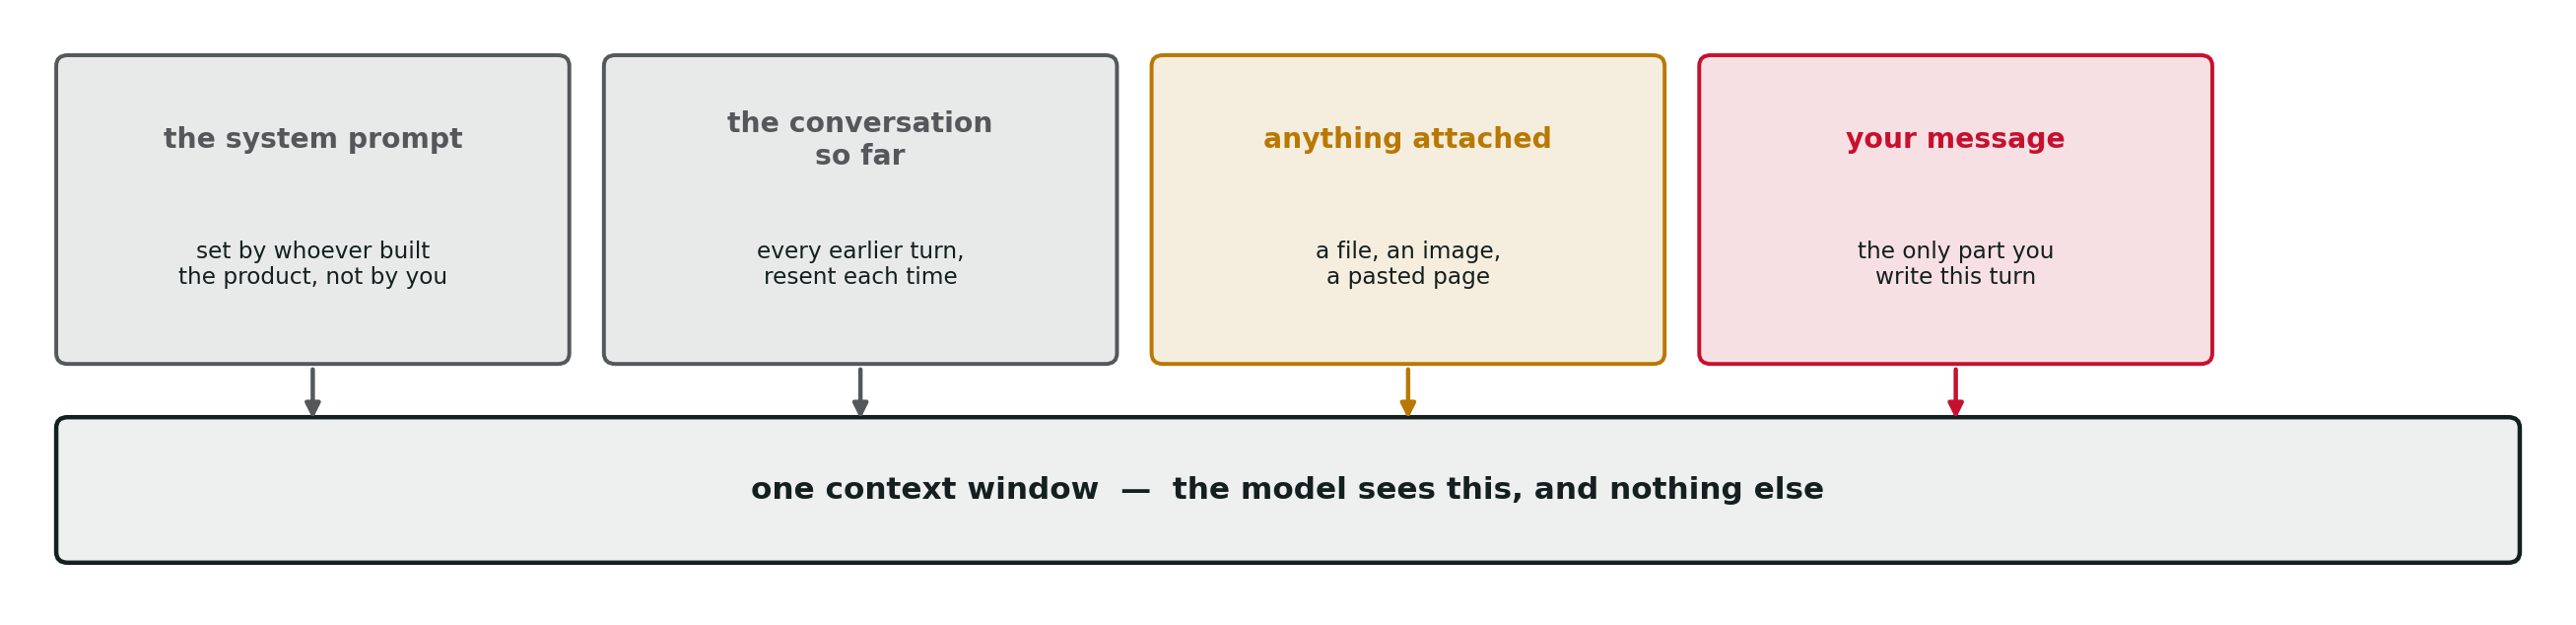
\includegraphics[height=34mm,width=\linewidth,keepaspectratio]{03-prompt-anatomy}\end{center}
  {\small Chapter 1 defined the \kw{context window}; Chapter 2 defined the \kw{system prompt}.
   Only the fourth box is written by the person at the keyboard, and three of the four are
   still there on every turn. Every lever in this chapter is a statement about one of these
   boxes.}
  \provenance{derived}
\end{frame}
\note{%
The anchor for the whole chapter. Point at each box and name who controls it.\\[0.3em]
The system prompt is set by whoever built the product. In the chat app that is the vendor; in
something built in-house it is the person who built it. Either way it is not the user, and it
is usually not visible.\\[0.3em]
Worth stressing: the conversation so far is resent in full on every turn. That is Chapter 1's
statelessness result, and it is why a long thread gets slower and more expensive.}

% ---------------------------------------------------------------- 4
\begin{frame}{Every lever in this chapter steers a dimension that was rated}
  \begin{center}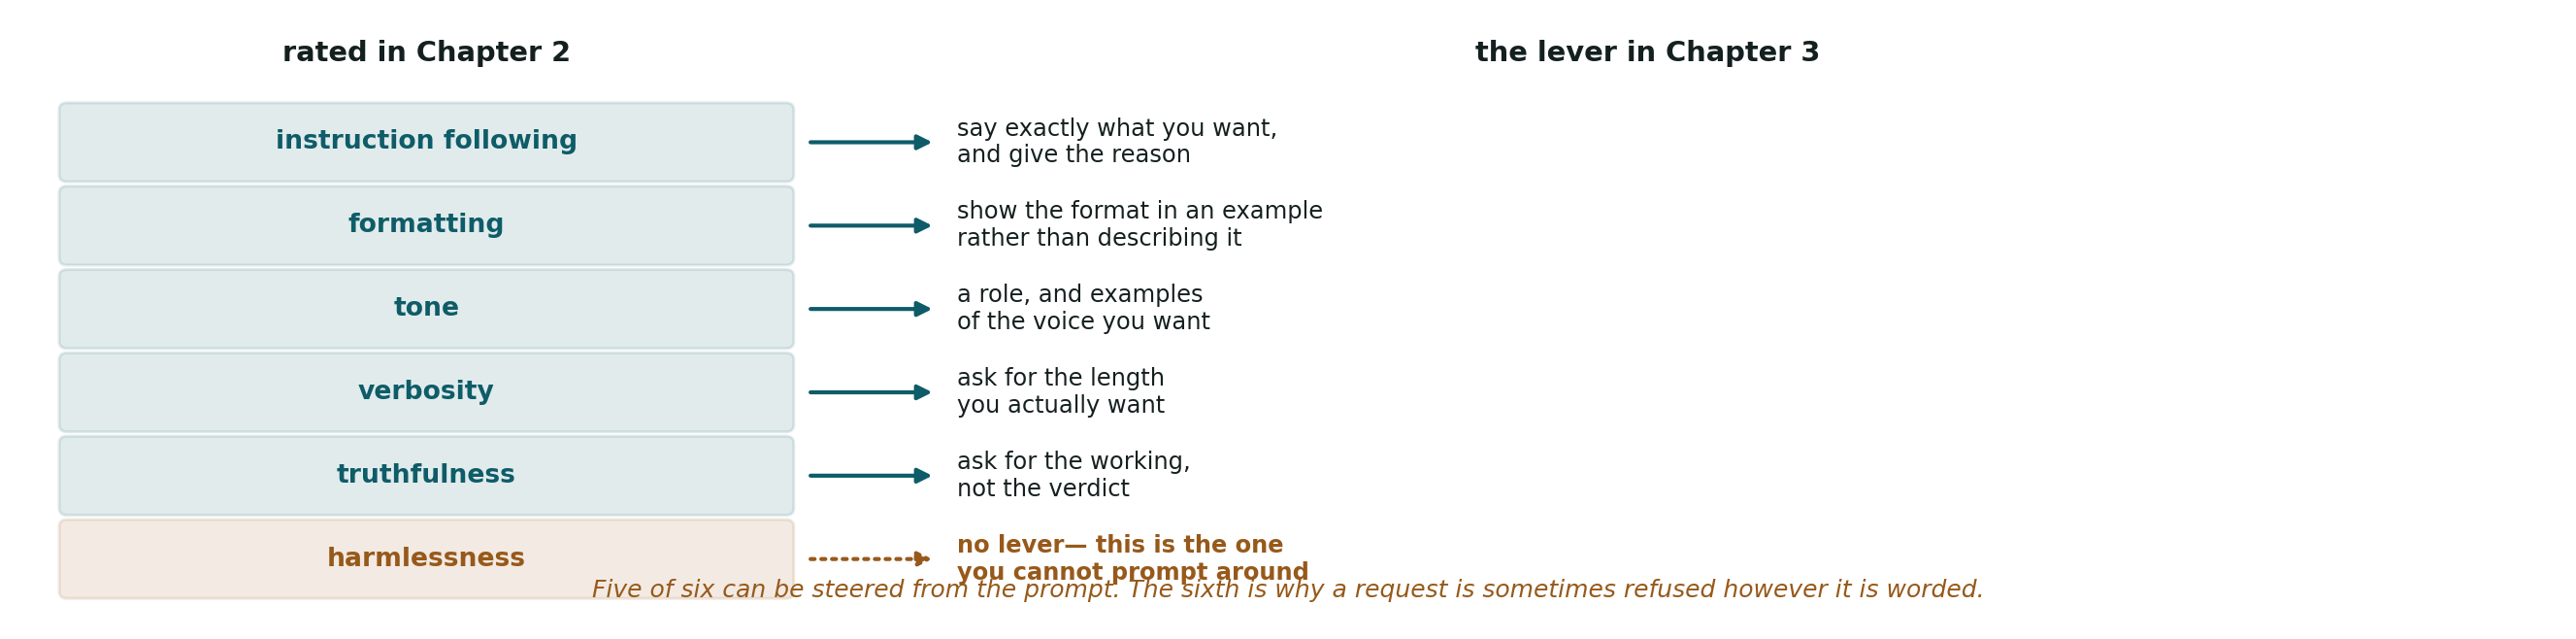
\includegraphics[height=34mm,width=\linewidth,keepaspectratio]{03-levers-map}\end{center}
  {\small The chapter walks this figure top to bottom. \kw{Harmlessness has no lever}, which
   is the informative row: a request refused on those grounds is refused however it is worded,
   and rephrasing to get around it is the one thing on this slide that does not work.}
  \provenance{derived}
\end{frame}
\note{%
The organising figure. Say plainly that the chapter follows it in order.\\[0.3em]
Spend the time on the last row. People assume every refusal is a phrasing problem, and try
increasingly elaborate wordings. Five dimensions are steerable; that one is not, by design,
and knowing which is which saves a great deal of wasted effort.\\[0.3em]
This also sets up Chapter 6, where the refusal boundary is the subject.}

% ---------------------------------------------------------------- 5
\begin{frame}{Prompt engineering assumes you already have a way to test the result}
  \begin{itemize}\small
    \item The vendor's own prompting guidance states its prerequisites before any technique:
          a clear definition of success, a way to measure against it, and prompts to improve.
    \item Without the second of those, every change on the following slides is a change whose
          effect you cannot observe.
    \item The failure this produces is specific. A prompt is edited, the next answer reads
          better, and the improvement is attributed to the edit rather than to sampling.
  \end{itemize}
  \begin{center}
  \begin{tikzpicture}[node distance=6mm]
    \node[uhghost]              (a) {success criteria};
    \node[uhghost, right=of a]  (b) {a way to test\\against them};
    \node[uhhi, right=of b]     (c) {then: prompt\\engineering};
    \node[uhamber, right=of c]  (d) {Chapter 4 builds\\the middle box};
    \draw[uhar] (a)--(b); \draw[uhar] (b)--(c); \draw[uhardot] (c)--(d);
  \end{tikzpicture}
  \end{center}
  \citesource{anthropic-prompting}
\end{frame}
\note{%
This is the strongest available argument for Chapter 4 and it comes from the vendor's own
prompting documentation, not from me. Say that out loud.\\[0.3em]
The room will recognise the failure mode immediately: it is the same one as tuning a model
until the plot looks right, without a held-out set.\\[0.3em]
Do not let this frame become a lecture on evaluation. Name the prerequisite, promise
Chapter 4, move on.}

% ---------------------------------------------------------------- 6
\begin{frame}{Saying exactly what you want removes the guesses the model would otherwise make}
  \begin{center}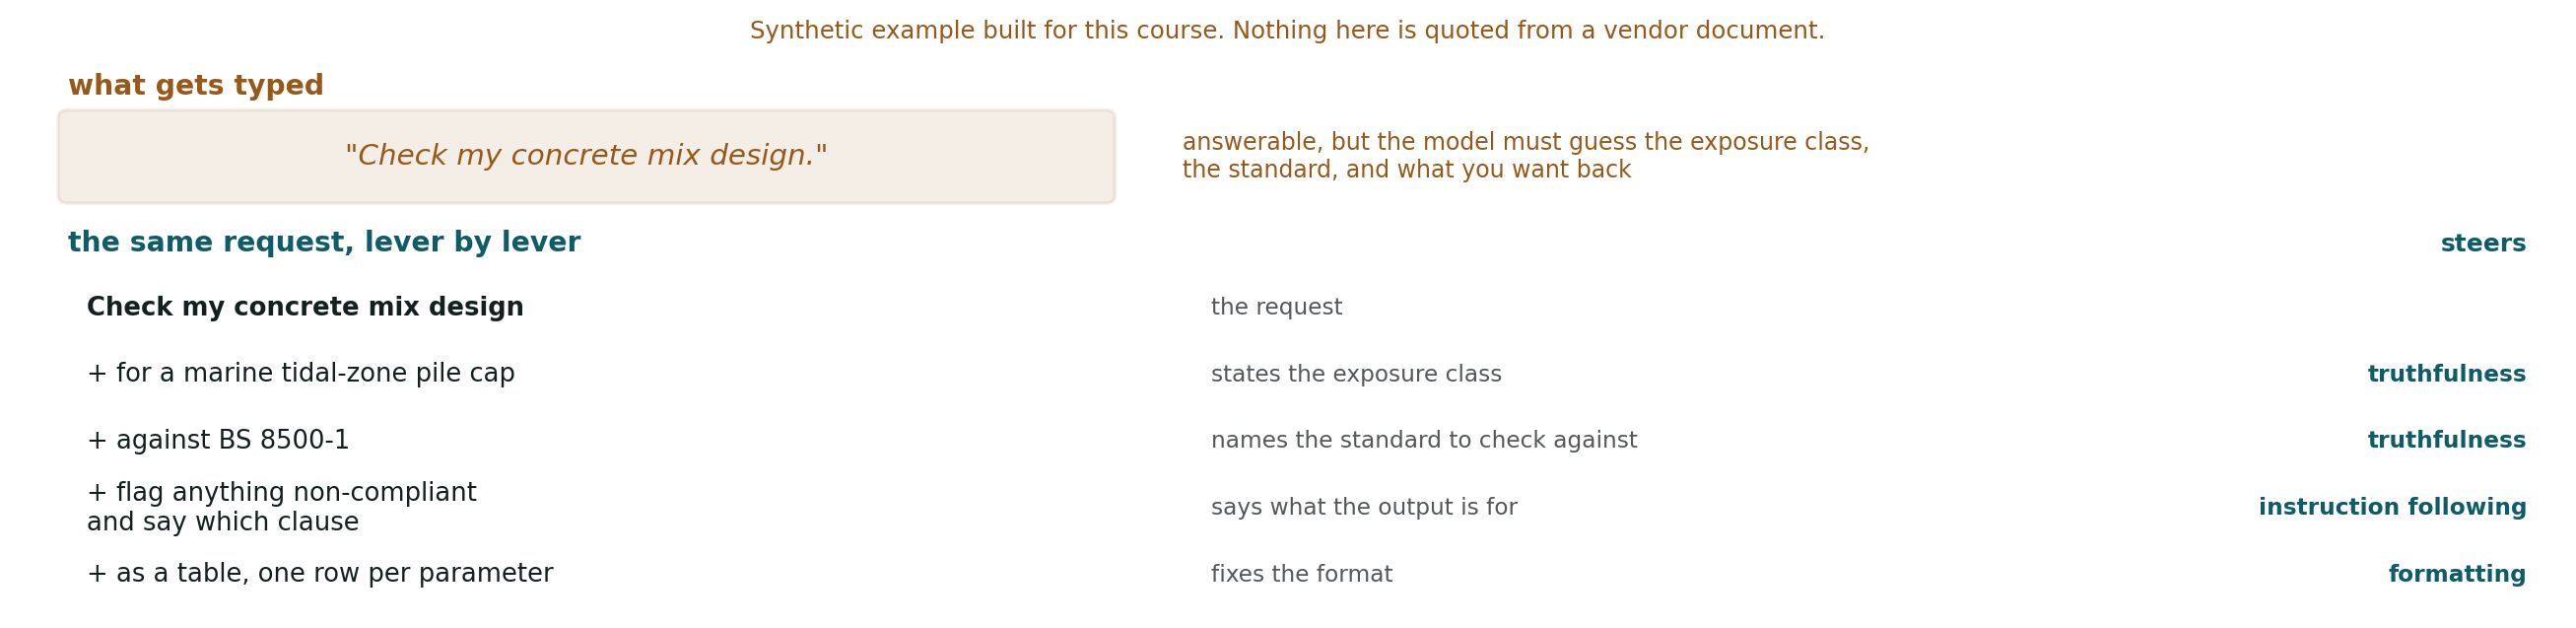
\includegraphics[height=33mm,width=\linewidth,keepaspectratio]{03-specificity}\end{center}
  {\small The weak version is answerable. It is answerable in several incompatible ways, and
   nothing in it says which one you meant, so the exposure class, the standard and the output
   format are all chosen for you.}
  \standing{documented, and each clause maps to a rated dimension.}
  \citesource{anthropic-prompting}
\end{frame}
\note{%
The running example for the chapter. Show the weak prompt first and ask the room what is
missing before revealing the improved version.\\[0.3em]
The engineering content is real: XS3 is the marine tidal-zone exposure class, and it drives
both the water/cement limit and the cover. Someone will check. That is the point of using
their own domain.\\[0.3em]
The right-hand column is the device the chapter runs on. Every clause is tagged with what it
steers, so this stops being a list of tips.}

% ---------------------------------------------------------------- 7
\begin{frame}{Giving the reason for a constraint makes it cover cases you did not list}
  \begin{columns}[T]
    \begin{column}{0.47\textwidth}
      {\footnotesize\color{uhslate}\textbf{constraint only}}\\[0.3em]
      {\small ``Use SI units.''}\\[0.6em]
      {\footnotesize Applies to the units. Says nothing about what to do with a figure quoted
       in psi, or a standard that is written in imperial.}
    \end{column}
    \begin{column}{0.47\textwidth}
      {\footnotesize\color{uhslate}\textbf{constraint with its reason}}\\[0.3em]
      {\small ``Use SI units, because this goes into a report that is checked against
       Eurocode.''}\\[0.6em]
      {\footnotesize Now covers the imperial-source case, the mixed-units case, and the
       question of which standard wins, none of which were listed.}
    \end{column}
  \end{columns}
  \vspace{0.6em}
  {\small The mechanism is the one Chapter 2 taught: instruction following was rated against
   the \kw{intent} of an instruction, not its literal surface, so a stated reason gives the
   model something to generalise from.}
  \standing{documented, with a stated mechanism.}
  \citesource{anthropic-prompting}
\end{frame}
\note{%
The most transferable idea in the chapter, and the one people under-use because it feels like
extra typing.\\[0.3em]
Analogy that lands with this room: a specification clause with its design intent stated is
easier to apply to a case the drafter did not foresee than a bare numeric limit. Same
principle.\\[0.3em]
The "why" is doing work at both ends. It also makes the prompt readable to the next person.}

% ---------------------------------------------------------------- 8
\begin{frame}{Tags separate the instruction from the data it applies to}
  \begin{columns}[T]
    \begin{column}{0.46\textwidth}
      {\footnotesize\color{uhred}\textbf{run together}}\\[0.4em]
      {\scriptsize\ttfamily Summarise this and flag any\\clause that conflicts with\\BS 8500
       The contractor shall\\ensure cover of not less than\\...}\\[0.5em]
      {\footnotesize Where the instruction stops and the document starts is a judgement call,
       and it is being made for you.}
    \end{column}
    \begin{column}{0.46\textwidth}
      {\footnotesize\color{uhteal}\textbf{separated}}\\[0.4em]
      {\scriptsize\ttfamily Summarise the document below\\and flag any clause that\\conflicts
       with BS 8500.\\[0.45em]{\color{uhteal}<document>}\\The contractor shall ensure...\\{\color{uhteal}</document>}}\\[0.5em]
      {\footnotesize The boundary is marked rather than inferred.}
    \end{column}
  \end{columns}
  \vspace{0.4em}
  {\small The tag names are arbitrary. What matters is that a boundary exists and that the
   same one is used consistently within a prompt.}
  \standing{documented, and this is also the defence Chapter 8 builds on.}
  \citesource{anthropic-prompting}
\end{frame}
\note{%
Short frame. The idea is obvious once seen and is skipped by nearly everyone.\\[0.3em]
Flag forward to Chapter 8: when the pasted document contains its own instructions, this
boundary is the difference between a summary and an injection. Do not teach injection here,
just plant it.\\[0.3em]
XML-style tags are conventional but nothing depends on the syntax. Headers or delimiters work.}

% ---------------------------------------------------------------- 9
\begin{frame}{Showing the format works better than describing it}
  \begin{itemize}\small
    \item A described format has to be interpreted before it can be produced, and an example
          skips that step.
    \item The guidance is specific about quantity and kind: three to five examples, relevant
          to the task, and diverse across the cases you care about.
    \item Diversity is the part usually skipped. Five examples of the same easy case teach
          the shape of the easy case.
  \end{itemize}
  \begin{center}
  \begin{tikzpicture}[node distance=6mm]
    \node[uhghost]             (a) {``return a table\\with the limits''};
    \node[uhbox, right=of a]   (b) {the model picks\\columns, order,\\units, precision};
    \node[uhhi, right=of b]    (c) {one worked row,\\written out};
    \node[uhamber, right=of c] (d) {every later row\\matches it};
    \draw[uhar] (a)--(b); \draw[uhar] (c)--(d);
  \end{tikzpicture}
  \end{center}
  \standing{documented, with stated bounds on how many and what kind.}
  \citesource{anthropic-prompting}
\end{frame}
\note{%
The count matters and people get it wrong in both directions. One example is a shape with no
variation; twenty is a large chunk of the window spent on formatting.\\[0.3em]
For this room: an example row of a compliance table, filled in with real values for a case
they know, is worth more than a paragraph describing the columns.\\[0.3em]
Diversity means spanning the cases, including the awkward one. If every example is a
compliant mix, the non-compliant output has no template.}

% ---------------------------------------------------------------- 10
\begin{frame}{A negative example puts the unwanted pattern into the window}
  \begin{itemize}\small
    \item The guidance is to say what to do rather than what to avoid, and the reason is
          mechanical rather than stylistic.
    \item Chapter 1 established that everything in the window is scored as context. An
          example of the output you do not want is still an example of that output.
    \item The replacement is not a softer prohibition. It is the positive instruction that
          makes the prohibition unnecessary.
  \end{itemize}
  \vspace{0.3em}
  \begin{columns}[T]
    \begin{column}{0.46\textwidth}
      {\footnotesize\color{uhred}``Do not write it as a bulleted list.''}
    \end{column}
    \begin{column}{0.46\textwidth}
      {\footnotesize\color{uhteal}``Write it as continuous prose, one paragraph per exposure
       class.''}
    \end{column}
  \end{columns}
  \standing{documented.}
  \citesource{anthropic-prompting}
\end{frame}
\note{%
The mechanism is worth stating carefully because it is counter-intuitive: a prohibition and
its subject arrive in the same window, and the window has no marker for "this is the bad
one".\\[0.3em]
Practical version: every "do not" in a prompt is worth rewriting once as a "do". Some cannot
be, and those are usually the ones that were load-bearing.\\[0.3em]
This is not absolute. A short prohibition next to a positive instruction is fine. A prompt
that is mostly prohibitions is the failure case.}

% ---------------------------------------------------------------- 11
\begin{frame}{The documentation claims a role changes tone and behaviour}
  \begin{itemize}\small
    \item What the guidance says a role in the system prompt does: focus \kw{behaviour and
          tone}. That claim is documented and this course accepts it.
    \item What people hear: that telling it to be a structural engineer makes it better at
          structural engineering. \kw{That is a claim about accuracy}, and it is a different
          claim.
    \item The two are separable, and there is a published result on the accuracy version.
          It is Chapter 4's, because it needs a measurement to settle rather than an argument.
  \end{itemize}
  \untested{the tone claim is documented. The accuracy claim is not established here — Chapter 4.}
  \citesource{anthropic-prompting}
\end{frame}
\note{%
Handle this one carefully. The room will have heard the persona advice from a dozen places
and half of them will use it.\\[0.3em]
Do not say it does not work. Say precisely what is claimed and by whom, and that the stronger
version is tested in Chapter 4 rather than asserted here.\\[0.3em]
If asked to preview: the published study covers many roles across several model families on a
factual question set, and finds no improvement over no persona. The caveat that matters is
that it is not this model on this domain, which is exactly why it is a Chapter 4 discussion
and not a Chapter 3 assertion.}

% ---------------------------------------------------------------- 12
\begin{frame}{Asking for a length is more reliable than asking for brevity}
  \begin{itemize}\small
    \item Verbosity was a rated dimension, so it moves. What moves it is a stated target
          rather than an adjective.
    \item ``Be concise'' is judged against whatever the rating layer settled on as concise.
          ``Two paragraphs, no preamble'' is not a judgement call.
    \item One version-specific caveat, and it is on the record: on the current model,
          responses run longer by default than on earlier ones, and the effort setting does
          not reliably shorten what you see. Prompting for length is the lever that works.
  \end{itemize}
  \standing{documented, including the version-specific caveat.}
  \citesource{anthropic-prompting}
\end{frame}
\note{%
Small frame, disproportionately useful. Most complaints about output length are fixed by one
clause.\\[0.3em]
The caveat is version-fragile and is flagged as such in references.md. Re-check it in the
week before delivery; if the behaviour has changed, the slide changes.\\[0.3em]
"No preamble" is worth calling out separately. A lot of perceived verbosity is the opening
restatement of the question.}

% ---------------------------------------------------------------- 13
\begin{frame}{The model decides how much to think, and wording biases that decision}
  \begin{center}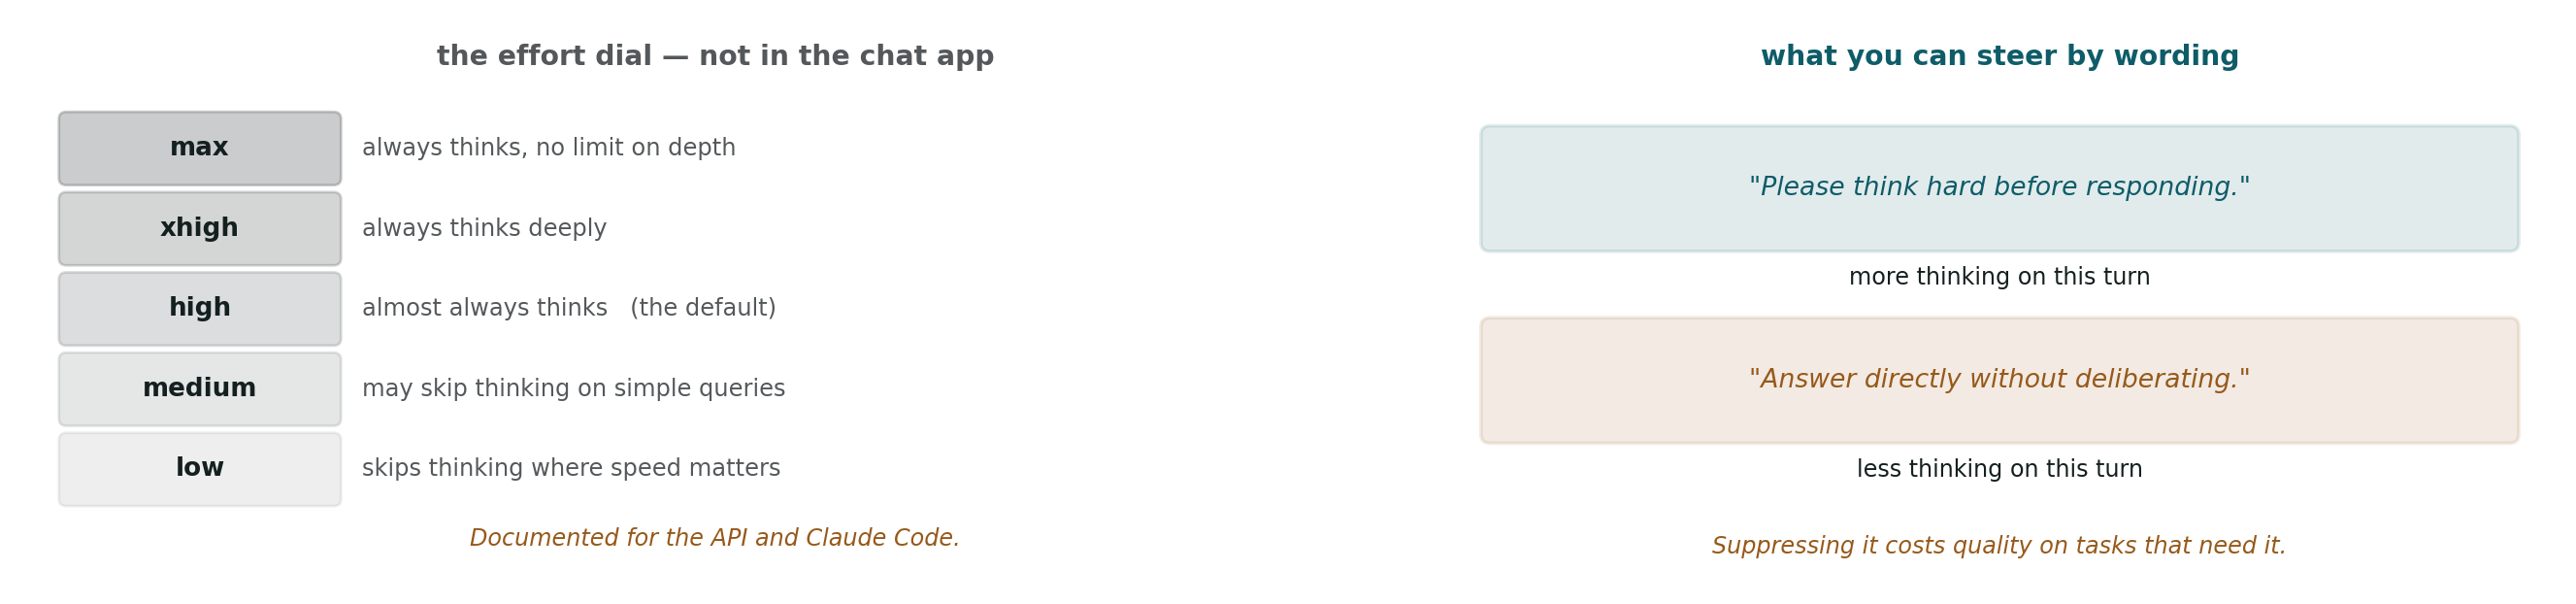
\includegraphics[height=33mm,width=\linewidth,keepaspectratio]{03-thinking-ladder}\end{center}
  {\small Thinking is decided \kw{per request}, by the model, on how hard the request looks.
   The effort ladder on the left is documented for the API and for the coding tool. In a chat
   window the lever is the wording, and the cost of suppressing thinking is borne on exactly
   the tasks that needed it.}
  \citesource{anthropic-thinking}
\end{frame}
\note{%
Correct a common belief here: thinking is not a switch the user holds. It is a decision the
model makes each turn.\\[0.3em]
Be honest about the split. The five-level dial is documented for the API and Claude Code. The
documentation does not put it in the chat app for the current models, so do not tell the room
it is there. What they have is the phrasing.\\[0.3em]
The warning on the right matters more than the technique: suppressing thinking is a real
quality cost on multi-step work, and the tasks where it helps are the ones where it is
slowest.\\[0.3em]
Second-order point worth making if there is time: thinking and the answer share one output
budget, so a long deliberation can crowd out the answer.}

% ---------------------------------------------------------------- 14
\begin{frame}{Asking for the working produces claims you can check}
  \begin{center}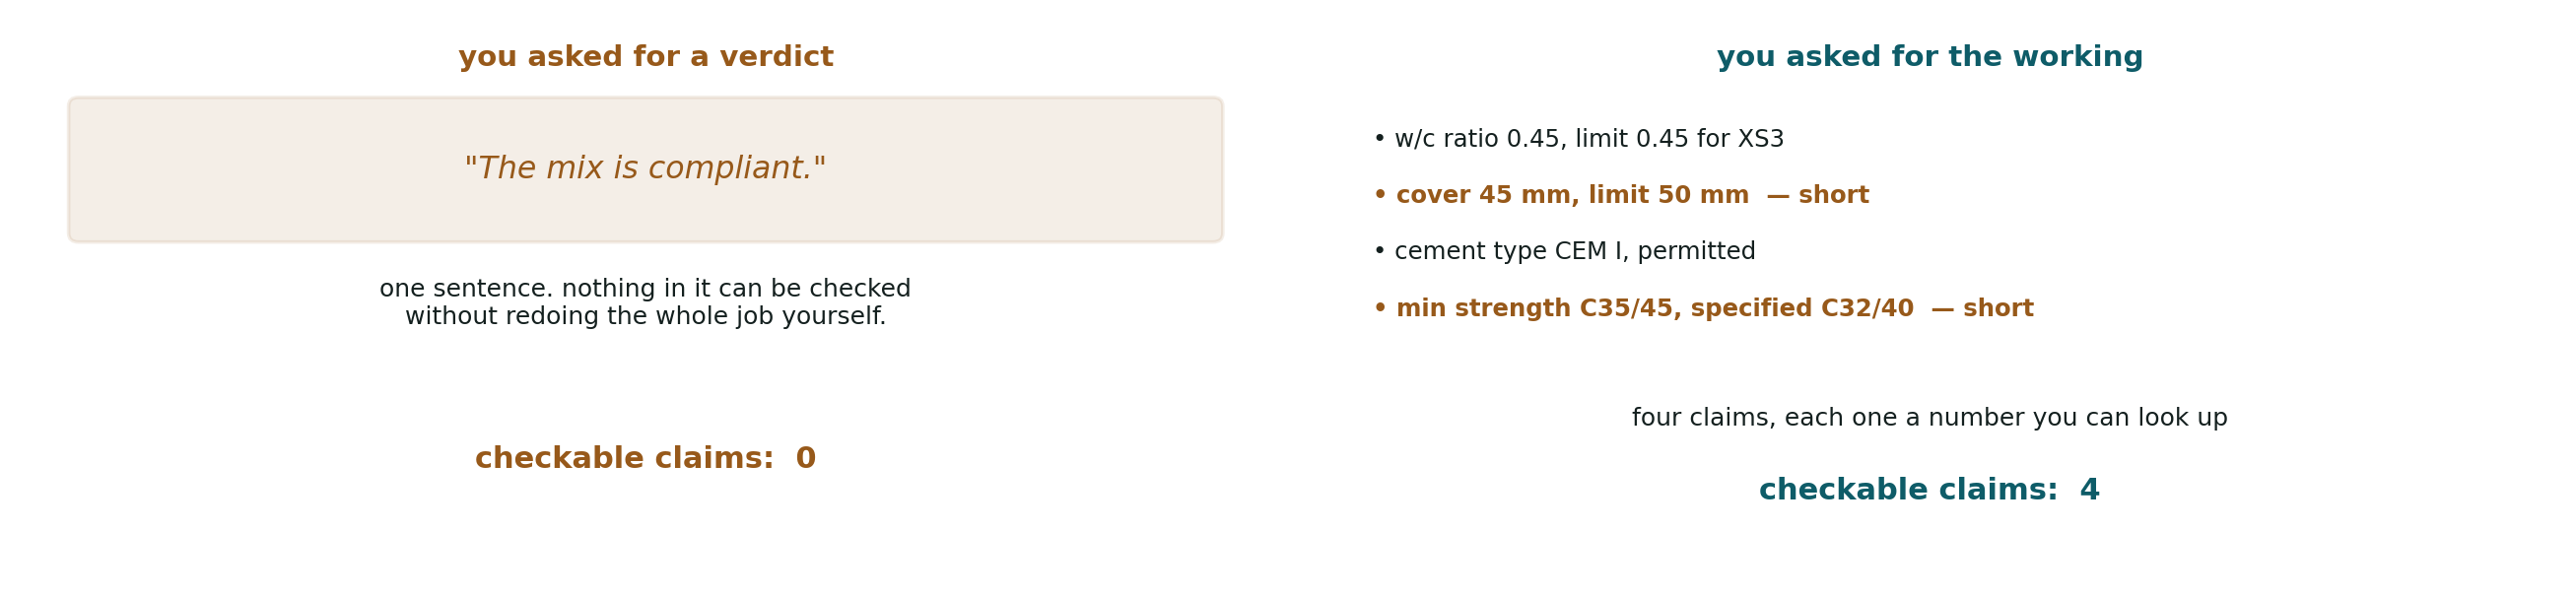
\includegraphics[height=32mm,width=\linewidth,keepaspectratio]{03-verdict-vs-working}\end{center}
  {\small Both answers cost about the same to produce. They differ in what they cost
   \kw{you}: the verdict has to be verified by redoing the work, and the working has four
   numbers that can each be looked up in a minute.}
  \standing{derived from the truthfulness dimension. The anti-pattern on the other side of it
   is frame 19.}
  \provenance{derived}
\end{frame}
\note{%
The most valuable habit in the chapter for this audience, and it is the one that transfers
directly to how they already work.\\[0.3em]
Frame it as the difference between a result and a calculation sheet. Nobody accepts a number
without the working from a junior engineer, and the reason is not distrust of the person.\\[0.3em]
The numbers on the right are synthetic but internally consistent: XS3 caps w/c at 0.45 and
sets a minimum cover, and the two flagged rows are the ones that fail.}

% ---------------------------------------------------------------- 15
\begin{frame}{Attaching the figure beats describing the figure}
  \begin{center}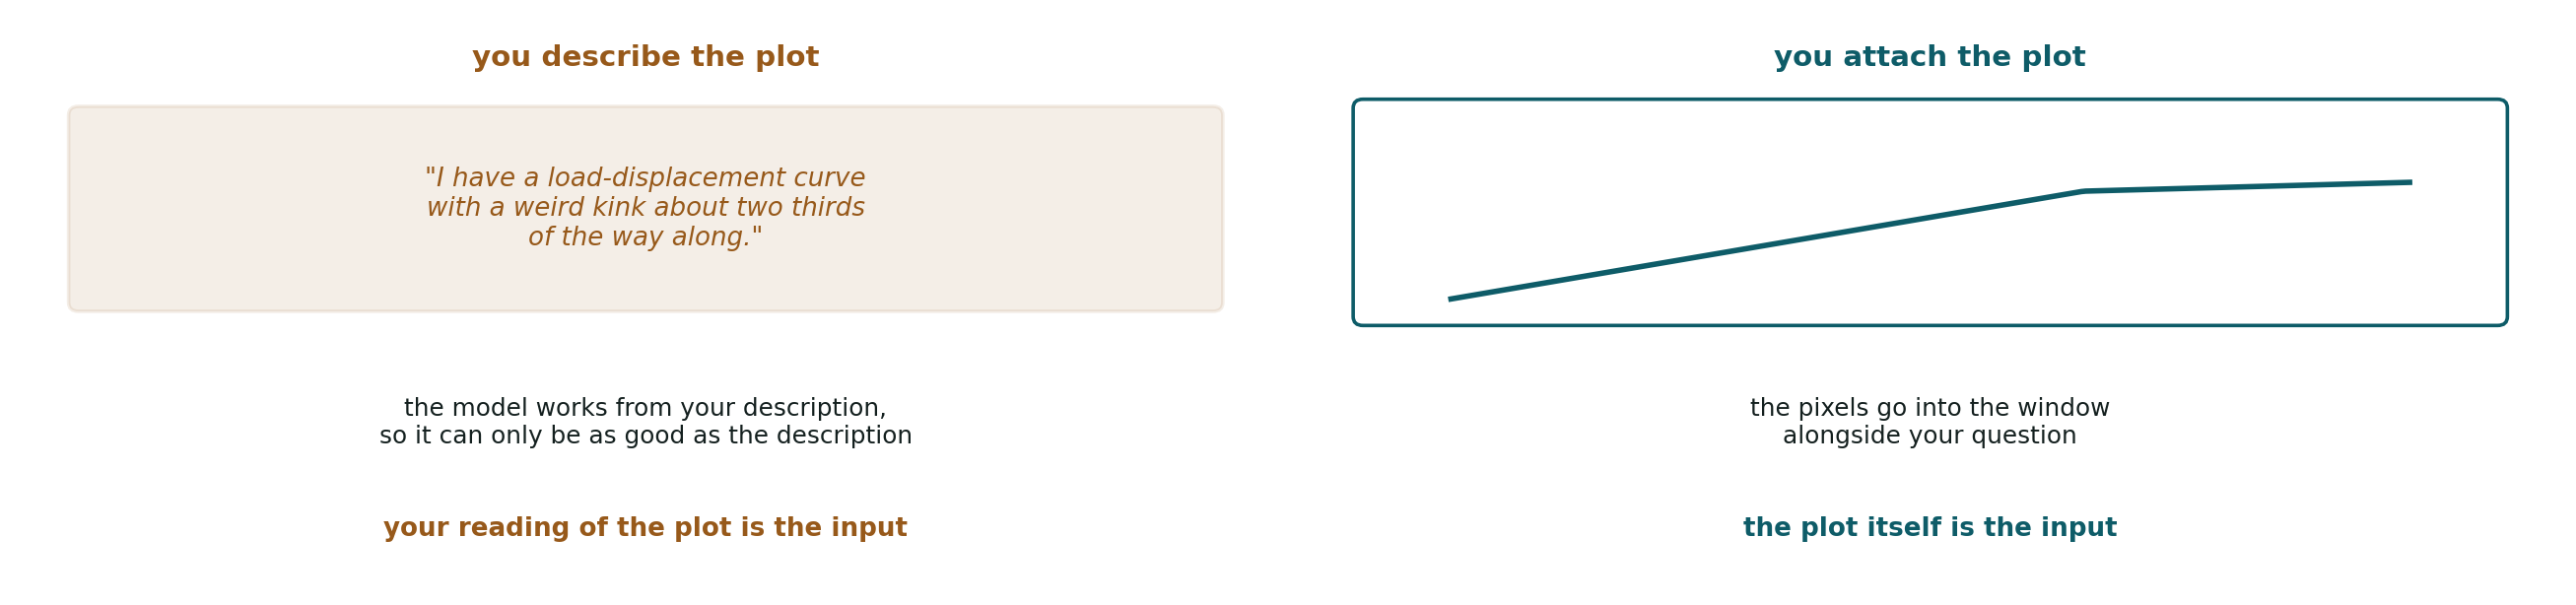
\includegraphics[height=30mm,width=\linewidth,keepaspectratio]{03-attachments}\end{center}
  {\small Chapter 1 established that the window takes images as well as text. A described plot
   is filtered through your reading of it first, so the answer is bounded by the description.
   An attached plot is not.}
  \standing{derived from Chapter 1's window definition. File-size limits are Chapter 14's.}
  \provenance{derived}
\end{frame}
\note{%
This is the largest gap in the old chapter and plausibly the highest-value lever this room
has. Photographs of cracked specimens, screenshots of a plot with an odd spike, a two-column
page of a paper.\\[0.3em]
The asymmetry is the teaching point. If you describe the kink, you have already decided it is
a kink and roughly where it is. If you attach the curve, that decision is still open.\\[0.3em]
Practical notes worth saying aloud: a screenshot of a table is worse than the table as text; a
photograph of a page is worse than the PDF. Attach the most direct form you have.\\[0.3em]
Chapter 14 covers what happens to a PDF on the way in, including that pages are converted to
images with the extracted text supplied alongside.}

% ---------------------------------------------------------------- 16
\begin{frame}{Every model has a date past which the literature is not in it}
  \begin{center}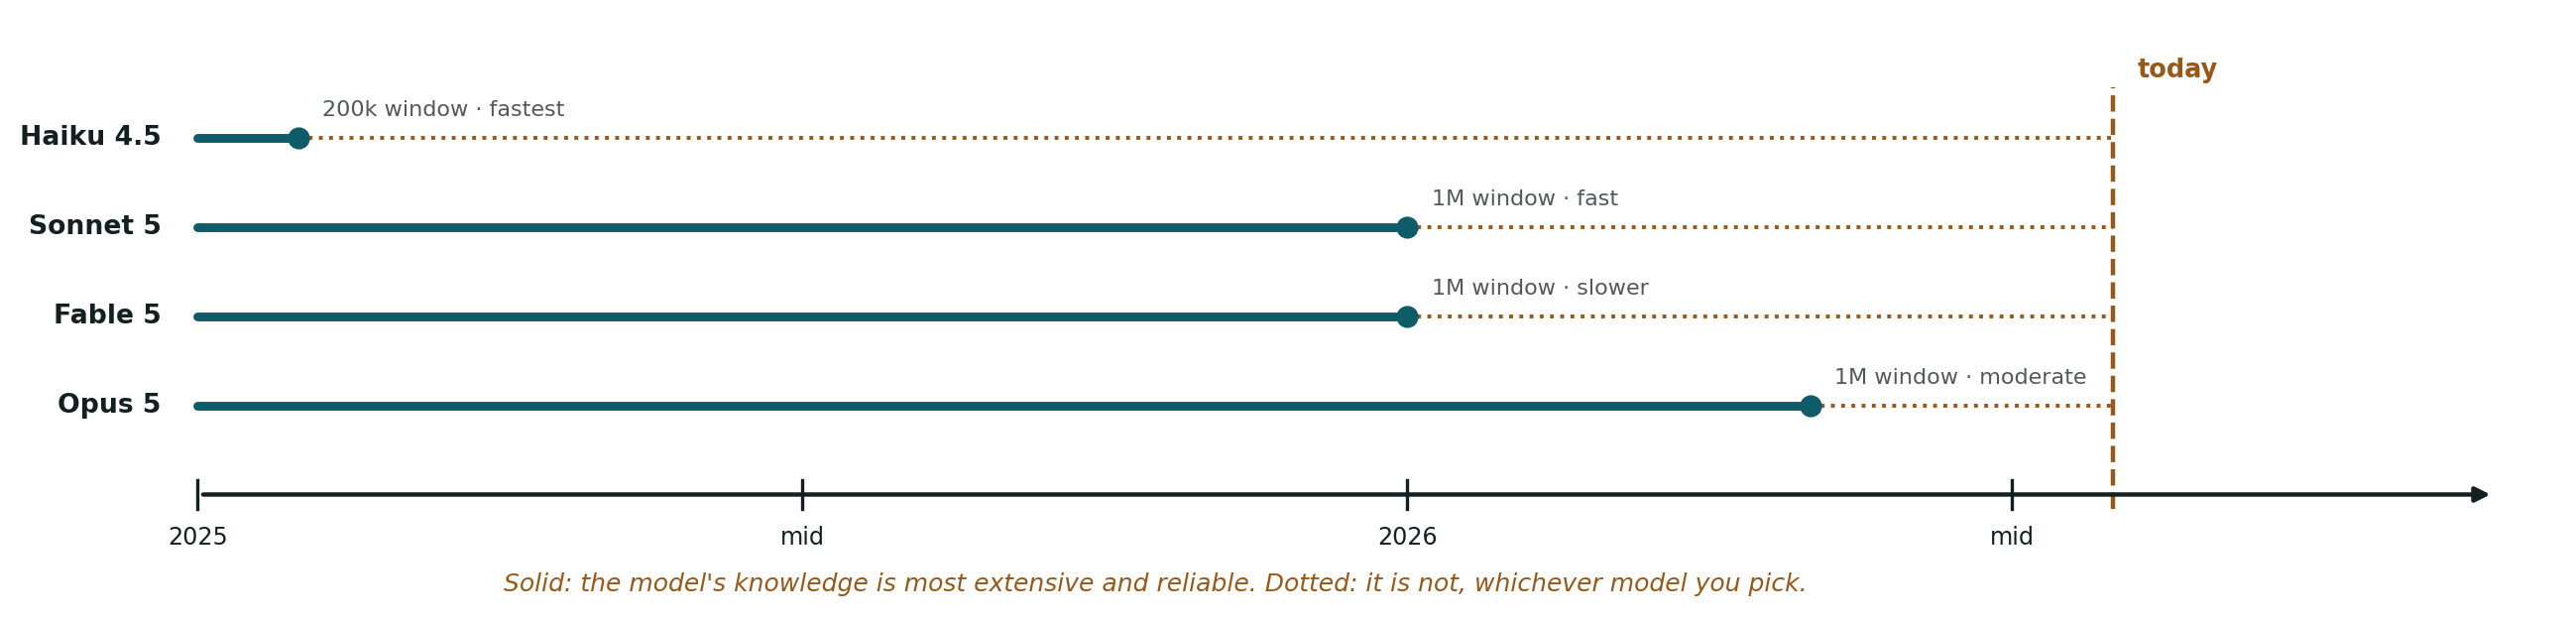
\includegraphics[height=33mm,width=\linewidth,keepaspectratio]{03-knowledge-cutoff}\end{center}
  {\small The picker offers models that differ in speed, in how much they hold at once, and in
   how recent their knowledge is. For literature work the third column is the one that decides
   an answer, and \kw{no choice in the list removes the dotted section}.}
  \citesource{anthropic-models}
\end{frame}
\note{%
The model-choice frame, and it is deliberately not a recommendation table. The vendor's own
default is to start with the most capable model, and for this room that is usually right, so
the interesting content is elsewhere.\\[0.3em]
The reliable knowledge cutoff is defined by the vendor as the date through which knowledge is
most extensive and reliable, and is distinguished from the broader training-data cutoff. Both
are published per model.\\[0.3em]
The consequence for this audience is direct: a question about a paper, a standard revision or
a code amendment after that date has no reliable answer from the model alone. That is what
search and attachment are for, and it is Chapter 9's subject.\\[0.3em]
Version-fragile. Re-fetch these dates in the week before delivery.}

% ---------------------------------------------------------------- 17
\begin{frame}{The anti-patterns pull the same levers backwards}
  \begin{center}
  \begin{tikzpicture}[node distance=6mm]
    \node[uhbox]               (a) {a rated\\dimension};
    \node[uhhi, right=of a]    (b) {pull the lever\\forward};
    \node[uhamber, below=8mm of b] (c) {pull it\\backwards};
    \node[uhwide, right=of b]  (d) {the behaviour\\you asked for};
    \node[uhwide, right=of c]  (e) {the behaviour\\that was rewarded};
    \draw[uhar] (a)--(b); \draw[uhar] (b)--(d);
    \draw[uhardot] (a)|-(c); \draw[uhar] (c)--(e);
  \end{tikzpicture}
  \end{center}
  {\small Three prompts follow that ask, without meaning to, for exactly the behaviour the
   rating layer rewarded. \kw{Each one is a lever from earlier in this chapter, reversed},
   which is why they are only visible now.}
  \provenance{derived}
\end{frame}
\note{%
The turn in the chapter. Everything so far has been a technique; the next three frames are
the same techniques misapplied.\\[0.3em]
State the position plainly rather than dramatically: the room is now on the other side of the
rubric from the raters in Chapter 2. What was rewarded is now what you have to avoid asking
for by accident.\\[0.3em]
This framing is only available because Chapter 2 came first.}

% ---------------------------------------------------------------- 18
\begin{frame}{A question containing its own answer gets that answer agreed with}
  \begin{columns}[T]
    \begin{column}{0.46\textwidth}
      {\footnotesize\color{uhred}\textbf{the answer is visible in the question}}\\[0.4em]
      {\small ``This mix fails because the water/cement ratio is too high, doesn't it?''}
    \end{column}
    \begin{column}{0.46\textwidth}
      {\footnotesize\color{uhteal}\textbf{the answer is not}}\\[0.4em]
      {\small ``Here is the mix design and the exposure class. Which parameters, if any, fall
       outside the limits?''}
    \end{column}
  \end{columns}
  \vspace{0.6em}
  {\small Agreement with the person asking was rewarded during rating. A question with a
   preferred answer in it is a request for that answer, and the reply reads as confirmation
   rather than as a check.}
  \standing{derived from Chapter 2's rating mechanism.}
  \provenance{derived}
\end{frame}
\note{%
The most common failure among people who already know their domain. You have a hypothesis, so
you phrase the question around it.\\[0.3em]
The damage is subtle. The answer is not wrong exactly; it is unexamined, and it arrives with
the confidence of a check that was never run.\\[0.3em]
Practical test to offer: before sending, read the question back and ask whether a reasonable
reader could tell which answer you are hoping for. If so, rewrite it.}

% ---------------------------------------------------------------- 19
\begin{frame}{A verdict is cheap to produce and impossible to check}
  \begin{itemize}\small
    \item Asking ``is this right?'' asks for a judgement with no working attached, and a
          confident judgement was the rated outcome.
    \item Nothing in a one-line verdict can be verified without redoing the task, so the
          verdict is either accepted on trust or discarded.
    \item The repair is frame 14, applied deliberately: ask for the parameters, the limits and
          the comparison, and reach the verdict yourself.
  \end{itemize}
  \vspace{0.3em}
  {\small Chapter 17 uses the same move as a technique rather than as a repair, on problems
   where the analysis is the deliverable.}
  \standing{derived. The reinforcement in Chapter 17 is deliberate.}
  \provenance{derived}
\end{frame}
\note{%
Pairs with frame 14 and it is worth saying that explicitly: this is the same lever, seen from
the failure side.\\[0.3em]
The reason this is hard to resist is that a verdict is what you actually want. The discipline
is asking for the thing that lets you produce the verdict.\\[0.3em]
Chapter 17 revisits this. Check the two frames read as reinforcement rather than repetition
when both are drafted.}

% ---------------------------------------------------------------- 20
\begin{frame}{Constraints that cannot all hold produce a silent drop}
  \begin{center}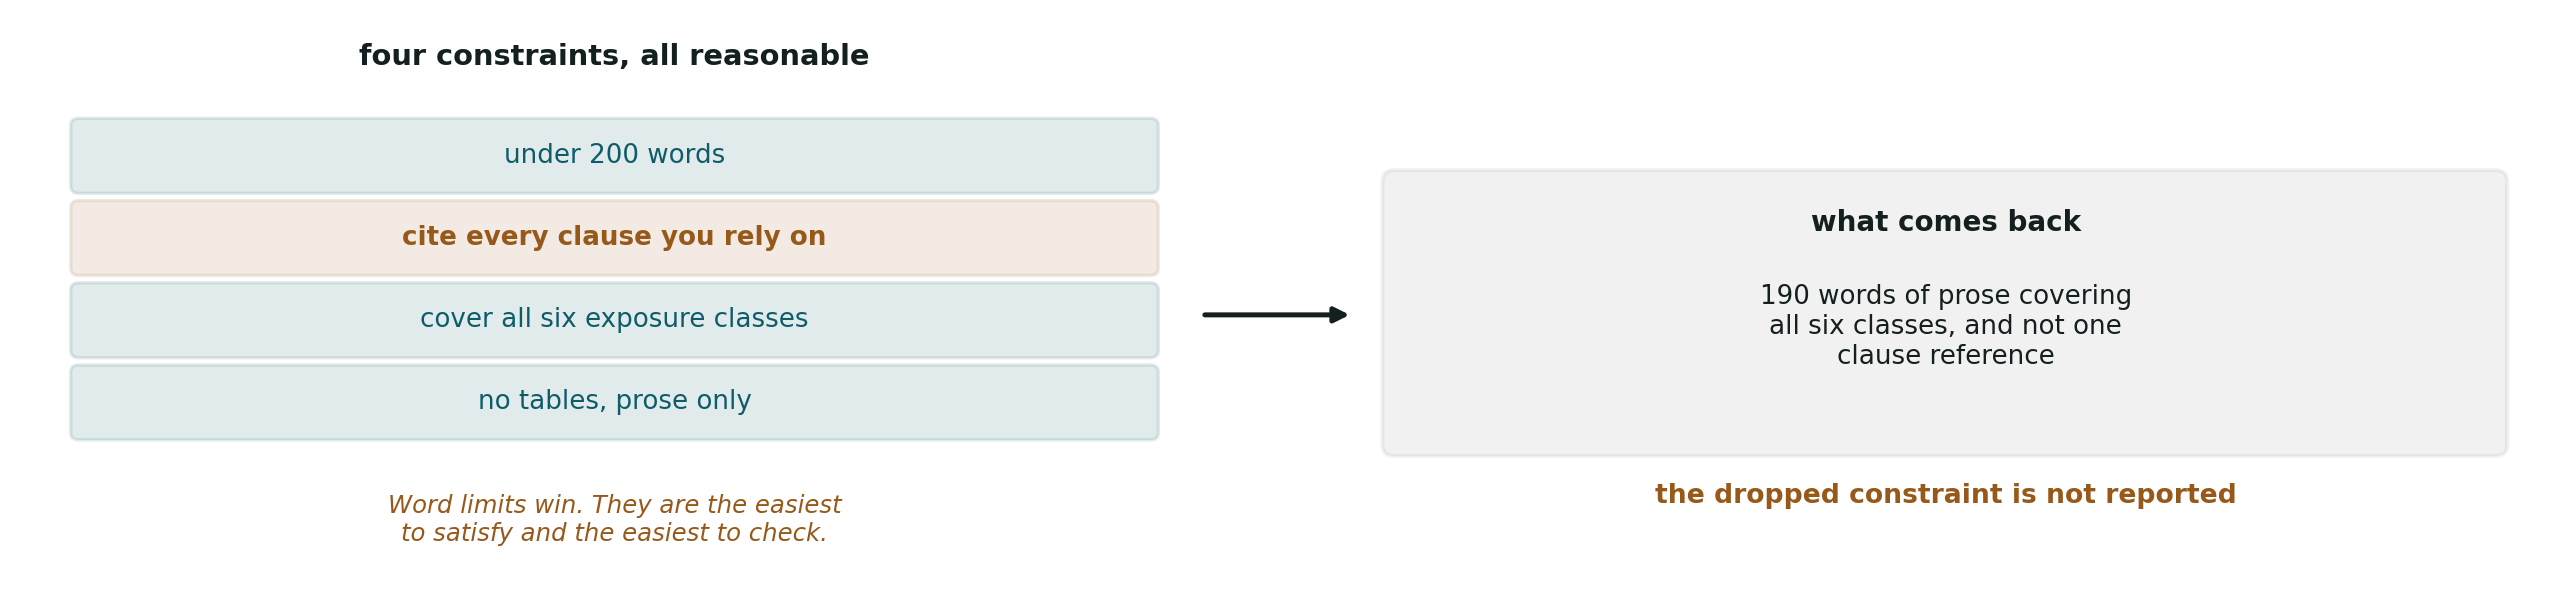
\includegraphics[height=29mm,width=\linewidth,keepaspectratio]{03-constraint-stack}\end{center}
  {\small Nothing in the output reports the dropped constraint, and the survivor is generally
   the one easiest to satisfy and to check. \kw{Ranking the constraints yourself} moves that
   choice back to you.}
  \standing{derived from Chapter 2's conflicting dimensions.}
  \provenance{derived}
\end{frame}
\note{%
Connect this to Chapter 2's rubric frame, where the dimensions were shown to conflict by
construction. This is that conflict arriving in the user's own prompt.\\[0.3em]
The practical repair is not fewer constraints. It is stating the order: say which one gives
first if they cannot all hold.\\[0.3em]
Word limits winning is a real and repeatable observation, and the reason is worth stating: a
word count is checkable by the model in a way that "cite every clause" is not.}

% ---------------------------------------------------------------- 21
\begin{frame}{A prompt tuned on one model is untested on another}
  \begin{itemize}\small
    \item The prompting guidance is explicitly model-specific, and already carries exceptions
          for the current model and a deprecation for an older mechanism.
    \item A prompt is tuned against one model's rating history. Another vendor's model has a
          different one, and so does the next version of the same model.
    \item The practical form: a prompt that has been working is evidence about the model it
          was working on, and the same prompt on a new model is an untested change.
  \end{itemize}
  \vspace{0.3em}
  {\small Chapter 12 treats portability as its subject. What this chapter needs is the habit
   of recording which model a prompt was tuned against.}
  \standing{documented.}
  \citesource{anthropic-prompting}
\end{frame}
\note{%
Under-appreciated and cheap to act on. Writing the model name and date at the top of a saved
prompt costs nothing and answers the question everyone eventually asks.\\[0.3em]
The vendor's own documentation carrying per-model exceptions is the evidence here, and it is
stronger than an assertion that prompts do not transfer.\\[0.3em]
Sets up Chapter 12. Do not pre-empt it.}

% ---------------------------------------------------------------- 22
\begin{frame}{Five of these are documented, and two are not yet established}
  \vspace{0.2em}
  {\footnotesize
  \begin{tabular}{@{}p{0.60\textwidth}p{0.34\textwidth}@{}}
    \textbf{What you can act on now} & \textbf{Standing} \\[0.2em]
    \hline\\[-0.7em]
    Say what you want; state constraints; give the steps in order &
      documented; maps to a rated dimension \\[0.25em]
    Explain why a constraint exists & documented, with a mechanism \\[0.25em]
    Separate instruction from data; 3--5 diverse examples &
      documented, with stated bounds \\[0.25em]
    Say what to do rather than what to avoid & documented \\[0.25em]
    A role changes \textbf{tone and behaviour} & documented \\[0.4em]
    \hline\\[-0.7em]
    A role improves \textbf{accuracy} & \textcolor{uhred}{\textbf{not established. Chapter 4.}} \\[0.25em]
    \emph{``Think step by step''} helps a current reasoning model &
      \textcolor{uhred}{\textbf{not established. Chapter 4.}} \\
  \end{tabular}}
  \vspace{0.2em}
  {\scriptsize The published chain-of-thought result used eight worked exemplars on a
   540-billion-parameter model of its day, which is a different proposition from four words
   typed at a model that already deliberates.}
  \citesource{wei2022}
\end{frame}
\note{%
The honesty frame, and the one to slow down on.\\[0.3em]
Say what the five documented rows rest on: one vendor's documentation about its own product.
That is the right primary source for how to steer that product, and it is still one company's
account of its own behaviour. It is why Chapter 4 exists.\\[0.3em]
The two red rows are the ones people arrive already believing. Do not settle them here.\\[0.3em]
On chain-of-thought: the paper is real, verified, and about few-shot exemplars in large models
of that generation. The four-word incantation is a folk descendant of it.}

% ---------------------------------------------------------------- 23
\begin{frame}{What we covered, and what is still open}
  \begin{columns}[T]
    \begin{column}{0.47\textwidth}
      {\usebeamercolor[fg]{frametitle}\bfseries What we covered}\\[0.5em]
      {\footnotesize
      A prompt is four things in one window.\\[0.35em]
      Five of the six rated dimensions have a lever; harmlessness does not.\\[0.35em]
      A stated reason generalises past the wording it was given in.\\[0.35em]
      Showing a format beats describing one.\\[0.35em]
      Thinking is the model's decision, biased by wording.\\[0.35em]
      The working can be checked; a verdict cannot.\\[0.35em]
      Three anti-patterns, each a lever reversed.}
    \end{column}
    \begin{column}{0.47\textwidth}
      {\usebeamercolor[fg]{frametitle}\bfseries What is still open}\\[0.5em]
      {\footnotesize
      Nearly all of the above rests on one vendor's documentation about its own product. Nothing
      here has been measured by us. \textbf{Chapter 4.}\\[0.5em]
      Two specific claims are flagged unsettled: that a role improves accuracy, and that a
      short reasoning instruction helps a current model.\\[0.5em]
      A prompt that works is evidence about one model on one day. \textbf{Chapter 12.}\\[0.5em]
      What happens when the document you pasted contains instructions of its own.
      \textbf{Chapter 8.}}
    \end{column}
  \end{columns}
  \provenance{none}
\end{frame}
\note{%
Close on the gap rather than on the techniques. The room now has a set of levers and no way to
tell whether any of them work on their own problems.\\[0.3em]
That is the handoff to Chapter 4, and it is the same shape as this chapter's own frame 5: the
prompting guidance assumed a test existed before any of this was applied.\\[0.3em]
Do not summarise the anti-patterns again. They were three frames ago.}

\end{document}
